\section{Technische Umsetzung}
\label{sec:technische_umsetzung}

%TODO identischer Inhalt mit Motivation
Ziel dieses Seminars war die Auslotung von Möglichkeiten die Daten öffentlich zugänglicher Quellen zu nutzen, um für fest definierte Untersuchungsgebiete erste Bewertungen der Verkehrssituation vorzunehmen. Diese Informationen können dazu dienen die Verkehrssituation auf einzelnen Streckenabschnitten zu untersuchen oder eine Bewertungsgrundlage zur Beurteilung bestehender Maßnahmen auf städtplanerischer Ebene zu schaffen. Vor allem in der Voranalyse kann dies Verkehrsplanern helfen einen ersten Überblick über die Verkehrssituation eines neuen Untersuchungsgebietes zu erhalten und damit erste Rückschlüsse auf Zusammenhänge und Problemfelder zuzulassen, die im Folgenden genauer untersucht werden können.\\

Das entwickelte Tool konzentriert sich auf die Ermittlung und Bewertung von öffentlich zugänglichen Verkehrsdaten und ermöglicht durch Momentaufnahmen und längere Untersuchungszeiträume eine erste Beurteilung der zeitlichen Entwicklung der Verkehrssituation innerhalb des definierten Untersuchungsgebiets. Angereichert werden diese Daten mit Flächeninformationen, die erste Rückschlüsse auf den Bebauungsgrad sowie die bestehende Infrastruktur geben und die zusätzlich zur Eingrenzung des Untersuchungsgebiets genutzt werden können.\\

Die Anforderungen jeder Untersuchung sind sehr individuell, weswegen bei der Entwicklung darauf geachtet wurde, dass stets sowohl bei der Datenerfassung wie auch der Datenanalyse die Untersuchungsparameter beim Programmaufruf eingestellt werden können. Somit ermöglicht das Tool sowohl makroskopische Betrachtungen wie beispielsweise die Bewertung der Verkehrssituation einer Stadt ebenso wie die Untersuchung ausgewählter Streckenabschnitte oder einzelner Straßen.

\subsection{Auswahl der verwendeten Kartendienste}
\label{sec:kartendienste}

Zur Erfüllung der individuellen Anforderungen musste auch der verwendete Kartendienst entsprechende Kriterien erfüllen, damit die Daten an die Untersuchung angepasst werden konnten.  Wichtigstes Kriterium war dabei der automatisierte Download des Kartenmaterials. Nur über einen automatisierten Prozess können zeitliche Verläufe -- vor allem über einen längeren Zeitraum -- zuverlässig aufgezeichnet und untersucht werden, die Generierung von Screenshots oder ähnliche Vorgehensweisen hätten diese Arbeit behindert. Aufgrund der Datenmenge und aufgrund rechtlicher Gründe stellt zudem kein Kartenanbieter sein vollständiges Kartenmaterial zur Verfügung, was dazu führt, dass Kartenausschnitte je nach Größe aus einzelnen Segmenten zusammengefügt werden müssen. Das genaue Vorgehen wird im Kapitel \ref{sec:kachelsystem} genauer beschrieben, es erfordert allerdings speziell bei der Verkehrsanalyse den synchronen Download mehrerer Aufnahmen und könnte manuell kaum geleistet werden. Neben der Automatisierung mussten zudem die Anforderungen der einzelnen Programmbausteine beachtet werden. Während bei der Flächenanalyse vor allem geometrisches Kartenmaterial benötigt wird, das mit der jeweiligen Flächennutzung verknüpft ist, ist bei der Verkehrsanalyse vor allem der Zugang zu aktuellen Schnappschüssen der Verkehrssituation wichtig.\\

Bei der Recherche geeigneter Kartendienste wurden die Anbieter \href{https://www.google.de/maps/}{GoogleMaps}, \href{https://www.bing.com/maps/}{BingMaps} und \href{http://www.openstreetmap.org/}{OpenStreetMap} untersucht. Alle drei Dienste stellen statische Schnittstellen bereit und ermöglichen damit den Download einzelner Kartensegmente mit unterschiedlichen Parametern. Zudem ist das Kartenmaterial aller drei Dienste -- innerhalb der jeweiligen Nutzungsbedingungen -- frei zugänglich und kann zum Zwecke des Seminars genutzt werden.\\

OpenStreetMap bietet sich als OpenSource-Map für wissenschaftliche Untersuchungen an, da das sehr genaue Kartenmaterial frei zugänglich und uneingeschränkt kostenfrei verfügbar ist. Die Karten entstehen dabei durch die Arbeit tausender freiwilliger Helfer, die den Genauigkeitsgrad der Karten stetig verbessern. Im Gegensatz zu kommerziellen Karten kann es zwar in abgelegenen Orten zu Lücken im Kartenmaterial kommen, die Anforderungen des Seminars beschränken sich allerdings auf die Analyse von Stadtgebieten und Infrastruktur, die Genauigkeit in diesen Gebieten kann vorausgesetzt werden. Auch wenn das Kartenmaterial umfangreich ist, bietet das System leider keine aktuellen Verkehrsinformationen an. Unabhängige Projekte wie \href{http://opentraffic.io/}{OpenTraffic} versuchen zwar diese Zusatzinformationen ebenfalls als OpenSource-Material zur Verfügung zu stellen, jedoch sind hier noch keinerlei Daten abrufbar (Stand März 2017), was die Daten auf die eigentlichen Kartendaten reduziert. Der Dienst würde sich daher sehr gut für die Flächenanalyse anbieten, der Fokus dieses Seminars lag allerdings in der Ermittlung und Analyse von  Verkehrsinformationen. Die Flächenanalyse dient primär der Voranalyse und der Einschätzung des Untersuchungsgebiets und wird daher vor allem für die Eingrenzung des Untersuchungsgebiets eingesetzt. Auch wenn über die bereitgestellten Schnittstellen Daten sehr feingranular ausgelesen werden können, wäre die Bestimmung einfacher Kennzahlen mit umfangreicher Einarbeitung und zusätzlichen Berechnungen zur Extraktion der Polygoninformationen verbunden gewesen.\\

Im Gegensatz zu OpenStreetMap bietet GoogleMaps eine sehr einfach justierbare und vor allem individuell anpassbare statische Schnittstelle \cite{googlestaticmap}, mit der das vorliegende Kartenmaterial per HTTP-Abruf in Bildform heruntergeladen werden kann. Mit Hilfe der URL-Parameter kann das Kartenmaterial an die Analyseanforderungen angepasst werden, dies reicht vom Aus- oder Einblenden bestimmter Inhalte bis hin zur individuellen Einfärbung ausgewählter Kartenflächen. Das resultierende Bildmaterial bietet einen schnellen wiederverwendbaren Ansatz das Untersuchungsgebiet einzuschätzen und eignet sich daher sehr gut für die Flächenanalyse, das genaue Vorgehen wird im Kapitel \ref{sec:area-analysis} detailierter beschrieben. Während GoogleMaps bei der Onlinenutzung dem Benutzer viele Einstellungs- und Interaktionsmöglichkeiten bietet, beschränkt sich der kostenlose Offline-Service im Wesentlichen auf das bereitgestellte Kartenmaterial. Zusätzliche Informationen in Form zusätzlicher Ebenen wie z.B. Verkehrsinformationen oder öffentliche Verkehrsnetze werden über die statische Schnittstelle seit einiger Zeit nicht mehr ausgeliefert und stehen ausschließlich dem dynamischen Kartensservice zur Verfügung. Wie bereits beschrieben wird allerdings der statische Download benötigt, um einen dauerhaften Service zu gewährleisten, demnach bietet der GoogleMaps-Dienst zwar sehr gut analysierbares Kartenmaterial, aber ebenso wie OpenStreetMap keine verwertbaren Verkehrsinformationen.\\

Microsofts Kartendienst BingMaps nutzt das Kartenmaterial von \href{https://here.com/}{Here} und bietet darüber viele Möglichkeiten auf Karten- und Verkehrsinformation zuzugreifen, im Gegensatz zu OpenStreetMap und GoogleMaps. Ebenso wie GoogleMaps bietete BingMaps eine anpassbare statische Schnittstelle \cite{bingstaticmap} über die das Kartenmaterial per HTTP-Abruf in Bildform heruntergeladen werden kann. Im Gegensatz zu den anderen untersuchten Diensten ermöglicht BingMaps die aktuellen Verkehrsinformationen im generierten Kartenabschnitt darzustellen, was eine dynamische Analyse des heruntergeladenen Materials ermöglicht. Mithilfe von Bildanalyseverfahren, wie im Kapitel \ref{sec:traffic-analysis} genauer beschrieben wird, kann somit die aktuelle Verkehrssituation sowie der Verlauf durch mehrfache Aufnahmen bestimmt und genutzt werden. Leider bietet BingMaps darüber hinaus nur bedingte Einstellungsmöglichkeiten, weshalb eine Flächenanalyse des vorliegenden Kartenmaterials unnötig erschwert werden würde.\\

Alle untersuchten Dienste bieten Vorteile, die nur kombiniert eine brauchbare Lösung für die Umsetzung des Tools bieten. Während die individuelle Einfärbung von GoogleMaps eine schnelle und reproduzierbare Flächenanalyse gewährleistet, bietet nur BingMaps Karten mit Verkehrsinformationen, aber keinen direkten Zugang zu den Nutzflächen. Die Kombination der beiden Dienste bietet zwar die notwendigen Daten, bringt allerdings zusätzliche Nachteile in der Nutzung mit sich. Sowohl GoogleMaps als auch BingMaps kostenlose Dienste unterliegen Nutzungbeschränkungen, die eine automatisierte Analyse behindern. Zum einen wird von beiden Anbietern die maximale Abfragemenge beschränkt und auf den Tag verteilt (GoogleMaps 25.000 Abfragen \cite{googleusagelimits}, BingMaps 30.000 Abfragen \cite{bingusagelimits}). Dies führt dazu, dass die Dienste durchschnittlich nur alle 2-3 Sekunden eine Anfrage durchlassen, der Abruf größerer Datenmengen wird dadurch deutlich erschwert. Zudem reduzieren beide Anbieter die verfügbare Bildqualität, was vor allem bei der Analyse größerer Flächen zu Problemen führt. Zu diesem Zweck wurde ein eigenes Kachelsystem entwickelt, was in Kapitel \ref{sec:kachelsystem} näher beschrieben wird. Mit diesem System war es möglich die Restriktionen der Kartenanbieter zu reduzieren und verwertbare Daten zu extrahieren ohne auf die kostenpflichtigen Dienste zurückgreifen zu müssen.\\

\subsection{Kachelsystem}
\label{sec:kachelsystem}

Die statischen Schnittstellen von GoogleMaps und von BingMaps liefern bei Aufruf das vorhandene Bildmaterial auf Grundlage der übergebenen Parameter. Wichtigster Parameter dieser Aufrufe ist der Mittelpunkt, der als Längen- und Breitengradangabe das Zentrum des resultierenden Bildes definiert. Über zusätzliche Parameter kann darüber hinaus die Höhe und die Breite des Bildes bestimmt werden. Die Bildgröße entscheidet maßgeblich darüber wie detailliert und umfangreich das Untersuchungsgebiet ist. Die bereitsgestellten maximalen Auflösungen (GoogleMaps maximal 640x640px \cite{googleusagelimits}, BingMaps maximal 2000x1500px \cite{bingstaticmap}) reichen allerdings in den meisten Szenarien nicht aus die untersuchten Flächen in ausreichender Auflösung darzustellen, damit eine weiterführende Analyse möglich ist.\\

GoogleMaps verwendet wie auch Here für ihre Karten die Mercator-Projektion. Mit Hilfe dieser Projektion werden die Breiten- und Längengrade in Pixelkoordinationen des Kartenausschnitts umgerechnet. Ausgehend von einer Basiskachel bei Zoomstufe 0 (siehe Abbildung \ref{fig:pixelcoordinates}) können damit alle Angaben in einen Gleitkomma-Pixelwert umgerechnet werden, der auf der Welt eindeutig ist. Will man nun die Karteninformationen um einen bestimmten Punkt darstellen, muss die Karte mit Hilfe eines Zoomfaktors vergrößert werden. In diesem Fall würde allerdings auch die Datenmenge exponentiell ansteigen, weswegen die Karten in jeder Zoomstufe in quadratische Kacheln zerlegt werden, die Koordinaten können dann eindeutigen Kachelkoordinaten zugeordnet werden.\\
\begin{figure}
\centering
\begin{tabular}{@{}cc@{}}
    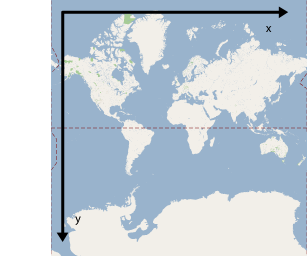
\includegraphics[height=6cm]{images/pixelCoordinates.png} &
    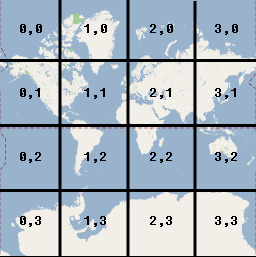
\includegraphics[height=6cm]{images/tileCoordinates.png} \\
\end{tabular}
\caption{Veranschaulichung der Basiskachel bei Zoomstufe 0 (links) und die Einteilung in Kacheln (rechts)}
\label{fig:pixelcoordinates}
\end{figure}

Ausgehend von diesen Überlegungen wurde ein Kachelsystem entworfen, welches von einem definierten Mittelpunkt in einer bestimmten Zoomstufe den Aufbau beliebig großer Kachelmatrizen ermöglicht und damit jedes Untersuchungsgebiet beliebig genau abbilden kann. Durch Hinzufügen weiterer Kachelebenen kann das Untersuchungsgebiet stetig vergrößert und an die Anforderungen angepasst werden. Jede Kachel wird mit der maximalen Auflösung erzeugt und bildet so die größte verfügbare Auflösung für die eingestellte Zoomstufe ab, durch Erhöhung der Zoomstufe kann die Genauigkeit bis zur maximal verfügbaren Zoomstufe (abhängig vom verfügbaren Kartenmaterial) erhöht werden. Dies ermöglicht die Generierung sehr feingranularer Bilder, die als Grundlage weiterer Untersuchungen dienen. Schichten können für ein bereits definiertes Zentrum jederzeit erweitert werden. Die Benamung der Kachelkoordinaten (siehe Abbildung \ref{fig:tilemap}) ausgehend vom Mittelpunkt ermöglicht es dem System bereits ermittelte Kacheln vorzuhalten und den Download neuer Schichten zu beschleunigen. Die statischen Schnittstellen unterstützen solche Kachelabfragen nicht, weswegen das Tool die Berechnungen der Mittelpunkte benachbarter Kacheln übernimmmt und sie selbstständig herunterlädt. Wie Kapitel \ref{sec:verfahrensentwicklung} am Beispiel Karlsruhe erläutert sollte genau auf den gewünschten Detailierungsgrad geachtet werden, denn mit jeder zusätzlichen Kachelschicht müssen $8(n-1)$ zusätzliche Kacheln heruntergeladen und analysiert werden, für eine komplette Kachelmatrix umfasst dies $(2n-1)^2$ Kacheln. Wie bereits in \ref{sec:kartendienste} beschrieben, kann dies zu einem deutlichen Mehraufwand führen und einige Zeit für den Download in Anspruch nehmen. Vor allem beim Einsatz in der Verkehrsanalyse (siehe \ref{sec:traffic-analysis}) sollte hier darauf geachtet werden, dass die Zeitspanne ausreicht alle Kacheln zu laden bevor ein weiterer Zeitschritt ansteht.
\begin{figure}
\centering
\begin{tabular}{@{}cc@{}}
    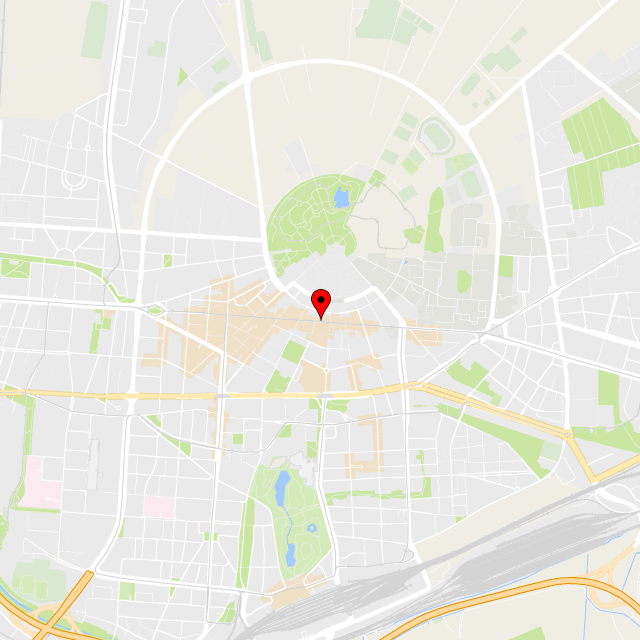
\includegraphics[height=6cm]{images/Karlsruhe_with_center.png} &
    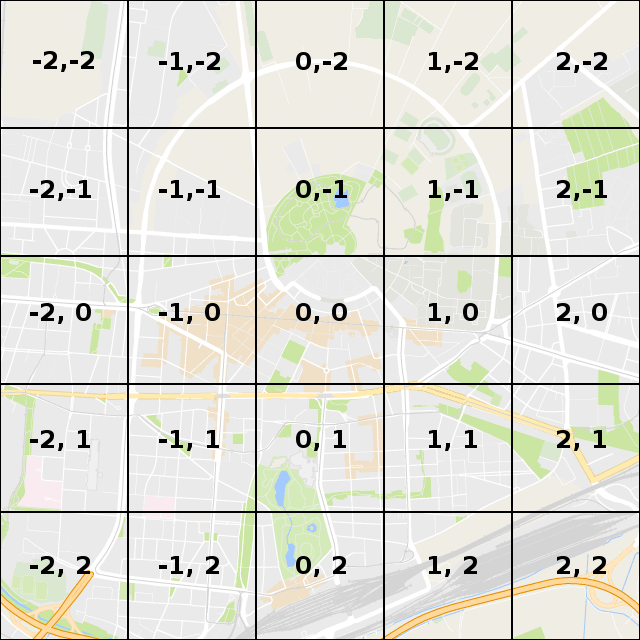
\includegraphics[height=6cm]{images/Karlsruhe_grid.png} \\
\end{tabular}
\caption{Kartenausschnitt der Stadt Karlsruhe mit Zentrumspunkt (links) und eingezeichneter Kachelmatrix (rechts)}
\label{fig:tilemap}
\end{figure}

\subsection{Flächenanalyse}
\label{sec:area-analysis}

Die Flächenanalyse dient der Voranalyse und Einschätzung des untersuchten Gebiets. Durch Anwendung der Analyse auf die einzelnen ermittelten Kacheln kann zudem eine Eingrenzung des Suchgebiets erreicht werden. Für die Ermittlung des Kartenmaterials kommt  die statische Schnittstelle von GoogleMaps zum Einsatz, da sich das System aufgrund seiner individuellen Einstellungsmöglichkeiten besonders dazu eignet die gewünschte Flächennutzung auszulesen. Folgende Kennwerte werden bei der Flächennutzung ermittelt:

\begin{itemize}\itemsep -2pt
\item Bebaute Fläche (man-made)
\item Naturfläche (nature)
\item Öffentlicher Verkehr (transit)
\item Straßen (road)
\item Autobahnen und Schnellstraßen (highway)
\end{itemize}

Zum Zwecke einer schnellen und direkten Analyse wurde der Ansatz der Karteneinfärbung genutzt. Dazu werden die umfangreichen Einstellungsmöglichkeiten der GooleMaps API genutzt, um jeden Flächentypen individuell einzufärben. Die API bietet dabei detaillierte Einflussmöglichkeiten auf die Flächeneinfärbung, die Darstellung der Beschriftungen sowie auf die Darstellung der Symbole und kann sehr gut den Bedürfnissen für die Bildanalyse vorbereitet werden. Eine darauf folgende Bildanalyse ermöglicht schnell Rückschlüsse auf die Anteile der Flächennutzung einzelner Kacheln wie auch des gesamten Untersuchungsgebiets. Abbildung \ref{fig:ka_area_analysis} zeigt einen Ausschnitt des Karlsruher Bahnhofs samt Umgebung, in der die unterschiedlichen Farbgebungen deutlich werden.\\

Das Tool übernimmt nach Übergabe der wichtigsten Einstellungsparameter die vollständige Analyse. Das System ermittelt in einem ersten Schritt die benötigten Kacheln und lädt sie (falls nicht bereits in einer vorherigen Analyse geschehen) über die Schnittstelle eingefärbt herunter. Die ermittelten Flächenanteile können direkt ausgegeben oder optional in eine CSV-Datei gespeichert werden. Die Generierung der angewendeten Kachelmatrix ermöglicht zudem eine schnelle Übersicht der analysierten Kacheln und ist im Ausschnitt \ref{fig:ka_area_analysis} ebenfalls erkennbar.

\begin{figure}
  \centering
    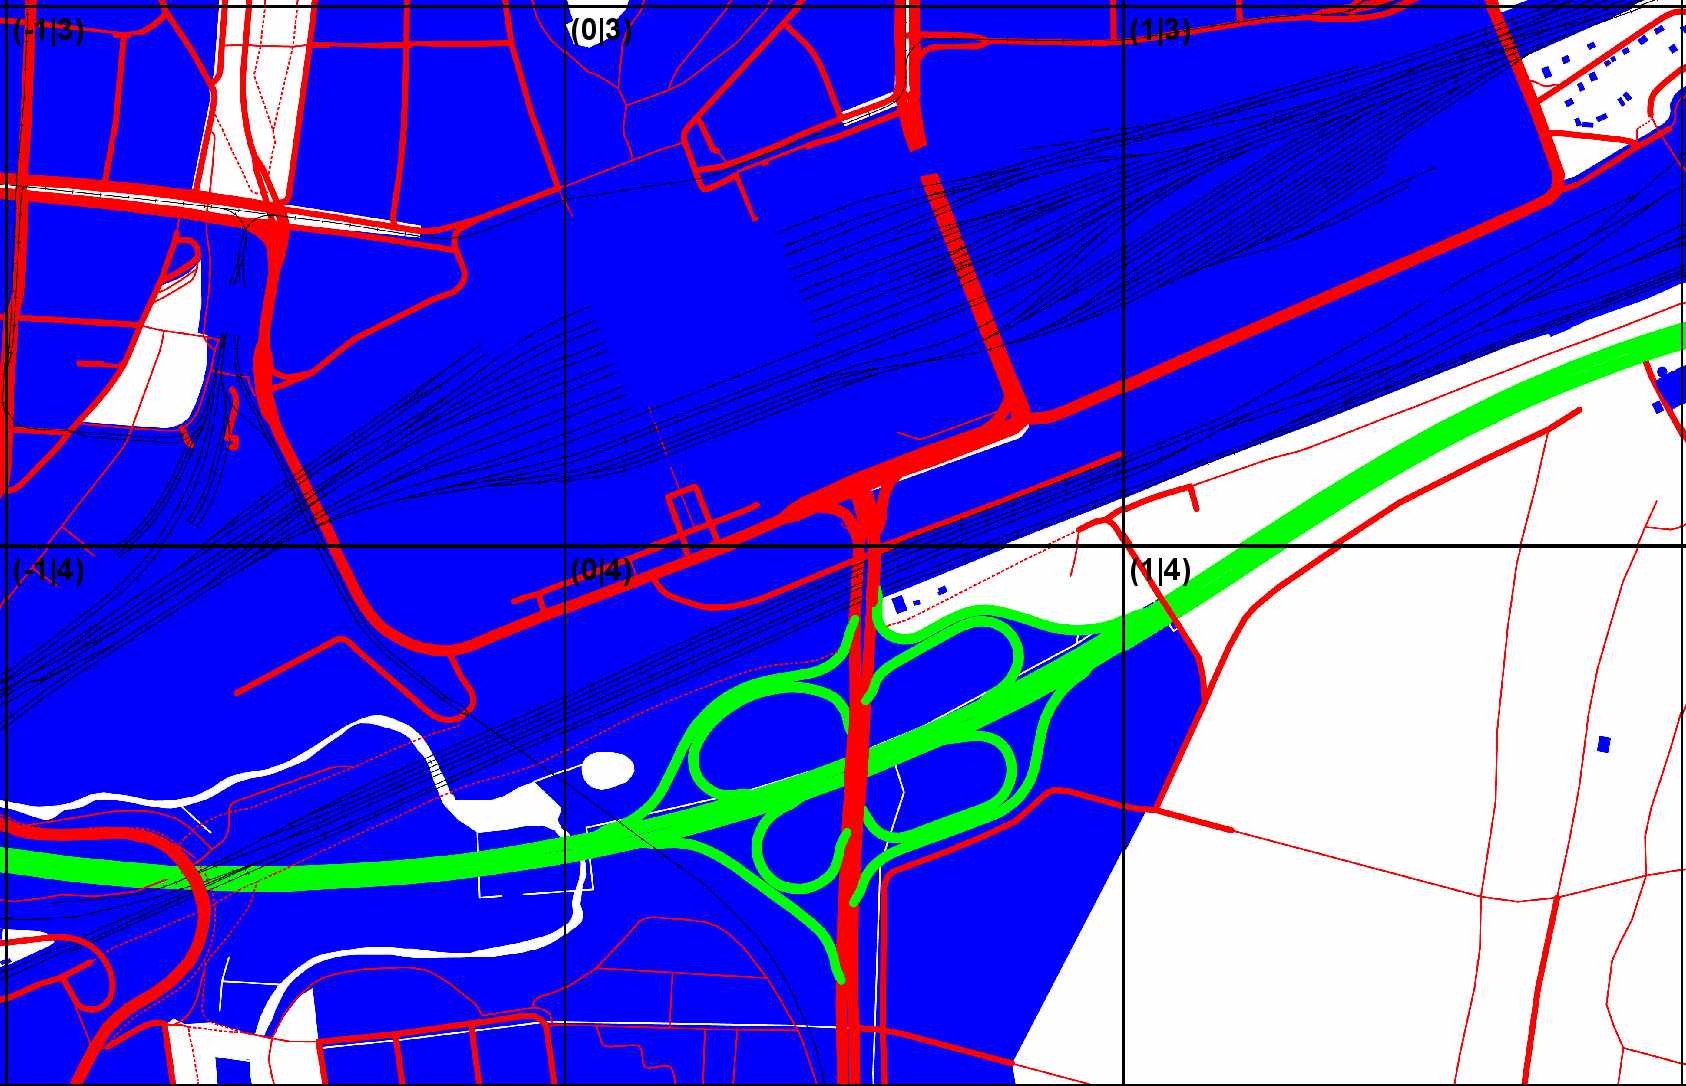
\includegraphics[width=0.75\textwidth]{images/karlsruhe_area_analysis_ausschnitt.png}
    \caption{Ausschnitt der Flächenanalyse der Stadt Karlsruhe auf Zoomstufe 17 und Kachelmenge 5}
    \label{fig:ka_area_analysis}
\end{figure}

\subsection{Verkehrsanalyse}
\label{sec:traffic-analysis}

Die Verkehrsanalyse wird genutzt um Momentaufnahmen oder zeitliche Verläufe der Verkehrssituation innerhalb des Untersuchungsgebiets zu erfassen und zu analysieren. Wie bereits in \ref{sec:kartendienste} gezeigt bietet nur der Kartendienst von BingMaps eine geeignete Schnittstelle, die Verkehrsinformationen per statischer Schnittstelle auszulesen. BingMaps bietet ebenso wie GoogleMaps einige Einstellungsmöglichkeiten beim Kartenabruf aber im Gegensatz zu GoogleMaps ist keine Einflussnahme auf die direkte Darstellung der Karte möglich. Da das Kartenmaterial nicht so effektiv verarbeitet werden kann wie das von GoogleMaps, muss die Verkehrsanalyse ohne zusätzliches Kartenmaterial auskommen, was in einem ersten Schritt mit dem der Flächenanalyse abgeglichen werden muss.\\

Beide Kartendienste arbeiten mit der Mercator-Projektion, wodurch das eingesetzte Kachelsystem (siehe \ref{sec:kachelsystem}) auf beide Systeme anwendbar ist. Die ermittelten Kacheln können daher auch bei BingMaps abgerufen werden und ermöglichen die direkte Verknüpfung mit den Flächenanalyseergebnissen. Davon ausgehend kann das System die momentane Verkehrssituation erfassen und lokal sichern. Abbildung \ref{fig:berlin_traffic} zeigt beispielhaft eine Momentaufnahme der Berliner Innenstadt, wie sie von BingMaps bereitgestellt wird. Die zusätzliche Verkehrsschicht wird über das zugrundeliegende Kartenmaterial geladen und farblich kodiert. Rot steht dabei für ein hohes, orange und gelb für ein mittleres sowie grün für ein niedriges Verkehrsaufkommen.

\begin{figure}
  \centering
    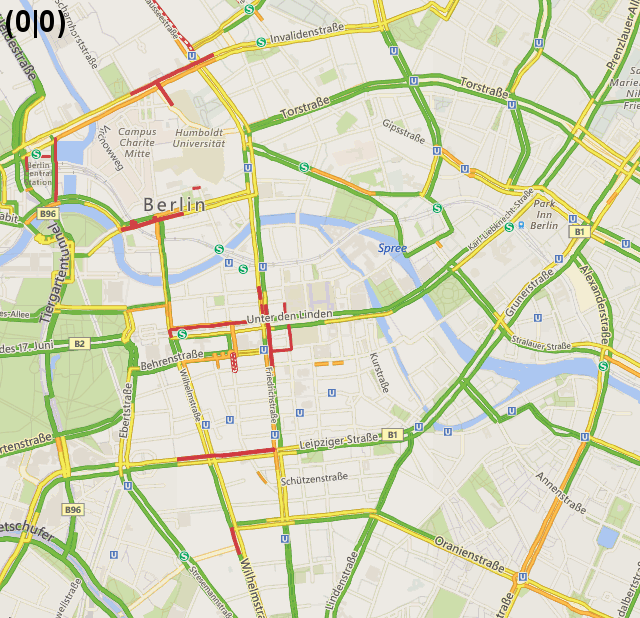
\includegraphics[width=0.45\textwidth]{images/traffic_berlin.png}
    \caption{Beispielhafte Kachel der Verkehrsinformationen zur Berliner Innenstadt (Zoomstufe 14)}
    \label{fig:berlin_traffic}
\end{figure}

Da das Ausgangsmaterial ausschließlich als Bild zur Verfügung steht, müssen die Daten über Bildanalyseverfahren extrahiert werden. Die Verkehrsinformation kann per Parameter aktiviert bzw. deaktiviert werden was den Zugriff auf die zugrundeliegende Karteninformation ermöglicht. Das Tool nutzt diesen Umstand, um von jeder Kachel zwei Bilder zu generieren und damit ein Differenzenbild zu berechnen. Dabei werden die beiden Aufnahmen verglichen und identische Farbwerte ignoriert, die abweichenden enthalten somit Verkehrsinformation. Die Genauigkeit der Differenz hängt stark vom Kartenmaterial ab, bereits leichte Veränderungen durch Hinzufügen der Verkehrsschicht können zu unerwartetem Rauschen führen. Ebenso sind die Farbwerte der Verkehrsinformationen nicht eindeutig definiert. Während in der Mitte meist ein ähnlicher Farbwert zu sehen ist, weicht dies vor allem in den Randgebieten deutlich voneinander ab. Zur Vermeidung von Bildrauschen und zur Vermeidung von Informationsverlust erfolgt die Segmentierung der Verkehrsinformationen mit einem Schwellenwertverfahren, das es ermöglicht über einen Schwellenwert auch ähnliche Farbwerte zu erfassen und einer bestimmten Verkehrsinformation zuzuordnen.\\

Bei der Berechnung werden alle Farbwerte in RGB-Kodierung (rot/gelb/blau) untersucht und dem jeweiligen Wert zugeordnet sobald alle Farbkanäle innerhalb des Schwellwertraums um einen gegebenen Farbwert liegen. Beispielsweise werden damit auch blasse Rottöne der Verkehrsinformat \textit{rot} zugeordnet. Je kleiner der Schwellwert desto näher müssen Farben am Ursprungswert liegen, blasse Farben werden ausgespart, die Information geht verloren. Je größer der Schwellwert desto mehr Farben werden zugeordnet obwohl diese vielleicht sehr weit vom eigentlichen Wert entfernt sind, es kann hier häufig zu Fragmenten im Ergebnisbild und zu fehlerhaften Zuordnungen kommen. Abbildung~\ref{fig:uebersicht_verkehrszustaende} stellt die Ergebnisse der Differenzberechnung unterschiedlicher Schwellwerte gegenüber. Bei niedrigem Schwellwert 5 werden deutlich weniger Punkte einer Verkehrsinformation zugeordnet was insgesamt zu deutlich dünneren Linien als im Original führt. Gerade an Stellen mit benachbarten Linien kann oft zu Lücken und fehlenden Informationen kommen. Im Gegensatz führt ein hoher Schwellwert 60 an einigen Stellen zu deutlichen erkennbarem Bildrauschen. Zudem ist die Tendenz zur Fehlerinterpretation im Bereich von gelb und orange ebenso erkennbar wie die Schriftzüge, die nach und nach zum Vorschein kommen, da deren Ränder dem darunterliegenden Farbwert oft sehr ähnlich sind. In den Untersuchungen des Seminars hat sich der Wert 30 als guter Näherungswert etabliert, bei dem ein sehr guter Detaillierungsgrad bei geringem Bildrauschen erreicht werden konnte. Wichtig ist allerdings bei jeder neuen Untersuchung den Wert zu überprüfen und verfälschte Ergebnisse zu vermeiden. Die Farbgebung des Kartenmaterial ist leider nicht weltweit konstant, was dazu führt, dass der Schwellwert nicht auf allen Karten ideal funktioniert. Vor allem im asiatischen Raum können damit nur bedingt Verkehrsinformationen ermittelt werden, hier muss mit deutlich höheren Werten gearbeitet werden\\

Einmal eingerichtet können die Einstellungen genutzt werden, um die vorliegende Datenmenge zu untersuchen. Das Tool berechnet anhand des ermittelten Differenzbild die Anteile der Verkehrsstärke und gibt diese Daten pro Untersuchungsgebiet oder pro Kachel aus. Im Zusammenspiel mit der Flächenanalyse (siehe \ref{sec:area-analysis}) kann damit der Stauindex des untersuchten Bereichs berechnet werden. Bei periodischem Programmaufruf kann das Tool zusätzlich genutzt werden automatisiert über einen beliebigen Versuchszeitraum Momentaufnahmen der Verkehrssituation zu generieren. Diese Datenmenge wird unabhängig von Schwellwert und anderen Einstellungen gespeichert, was eine nachträgliche Analyse mit abweichenden Parametern ermöglicht. Die Ausgabe als animierte GIF-Datei dient dabei der schnellen Visualisierung des beobachteten Verkehrsverhalten und ermöglicht erste Rückschlüsse auf Ursachen und Problembereiche. Der CSV-Export ermöglicht die weitere Verarbeitung und Untersuchung in anderen Softwareprodukten.

\begin{figure}
\begin{tabular}{@{}cc@{}}
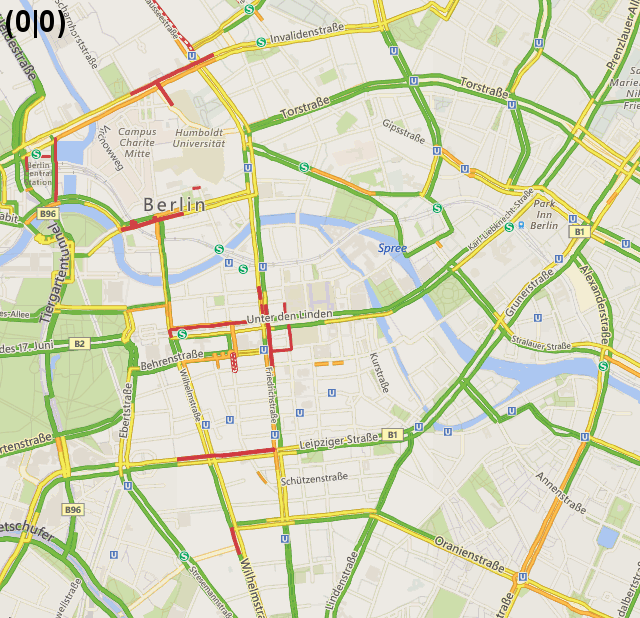
\includegraphics[width = 0.48\textwidth]{images/traffic_berlin.png} &
\includegraphics[width = 0.48\textwidth]{images/traffic_berlin_t5.png} \\ 
\textbf{Originalbild}  & \textbf{Schwellwert=5}   \\\\
\includegraphics[width = 0.48\textwidth]{images/traffic_berlin_t30.png} & 
\includegraphics[width = 0.48\textwidth]{images/traffic_berlin_t60.png} \\
\textbf{Schwellwert=30} & \textbf{Schwellwert=60}\\
\end{tabular}
\caption{Differenzbilder zur Segmentierung der Verkehrsinformationen bei unterschiedlichen Schwellwerten}
\label{fig:uebersicht_verkehrszustaende}
\end{figure}
